\documentclass{article}

\usepackage{mathtext}
\usepackage[T2A]{fontenc}
\usepackage[utf8]{inputenc}
\usepackage[english, russian]{babel}
\usepackage[pdftex]{graphics}
\usepackage{tikz}
\usepackage{array}
\usepackage[left=1cm,right=1cm, top=2cm,bottom=2cm,bindingoffset=0cm]{geometry}
\usepackage{gensymb}

\usepackage{subfigure}

\usepackage{graphicx}
\DeclareGraphicsExtensions{.pdf,.png,.jpg}

\begin{document}

\textbf{2.7. Отличия ДНК от РНК}

\begin{enumerate}
\item Мономерная единица ДНК --- дезоксирибонуклеотид, РНК --- рибонуклеотид.
\newline
Рибонуклеотид образован рибозой, азотистым основанием и остатком фосфорной кислоты. Рибоза --- пятиуглеродный моносахарид. Рибоза, входящая в состав биологических структур, обладает свойством хиральной чистоты: молекулы РНК построены исключительно на «правой» рибозе.
\newline
Дезоксирибонуклеотид образован дезоксирибозой, азотистым основанием и остатком фосфорной кислоты. Дезоксирибоза --- производное рибозы, где гидроксильная группа у второго атома углерода замещена водородом с потерей атома кислорода (дезокси --- отсутствие атома кислорода).
\newline
Таким образом, у рибозы есть дополнительная, по сравнению с дезоксирибозой, гидроксильная группа. Эта группа увеличивает вероятность гидролиза молекулы, то есть уменьшает стабильность молекулы РНК.

\item Азотистые основания в молекуле ДНК – тимин, аденин, цитозин, гуанин; в РНК же комплементарный аденину нуклеотид --- не тимин, а урацил --- неметилированная форма тимина.

\item Отличаются функции молекул. ДНК является матрицей для транскрипции, она хранит генетическую информацию. Основная функция молекулы ДНК в клетках --- точное сохранение информации о строении белков и РНК. РНК же участвует в синтезе белка: информационная РНК (иРНК) синтезируется на основе ДНК в ходе транскрипции, после чего, в свою очередь, используется в ходе трансляции как матрица для синтеза белков; транспортная РНК (тРНК) отвечает за доставку аминокислот к рибосомам; рибосомная РНК является составляющей рибосом, она считывает информацию с иРНК и катализирует образование пептидных связей между присоединёнными к тРНК аминокислотами. У молекул РНК есть и другие функции: например, малые ядерные РНК принимают участие в сплайсинге эукариотических матричных РНК и других процессах. 
\newline
Есть исключение: РНК является составной частью геномов большинства вирусов, у которых она выполняет ту же функцию, что и ДНК у высших организмов.

\item ДНК существует в форме двойной спирали, состоящей из двух отдельных молекул. Молекулы РНК, в среднем, гораздо короче и преимущественно одноцепочечные. Структурный анализ биологически активных молекул РНК, включая тРНК, рРНК и другие молекулы, которые не кодируют белков, показал, что они состоят не из одной длинной спирали, а из многочисленных коротких спиралей, расположенных близко друг к другу и образующих нечто, похожее на третичную структуру белка. В результате этого РНК может катализировать химические реакции, например, пептидил-трансферазный центр рибосомы, участвующий в образовании пептидной связи белков, полностью состоит из РНК.

\end{enumerate}

\textbf{2.8. Параметры, характеризующие глобальное потепление}
\begin{enumerate}

\item \textbf{Средняя приповерхностная температура воздуха}
\newline
За период 1901-2012 гг. она выросла на $(0,89 \pm 0,20) \degree C$. Данные о динамике средней годовой температуры на планете можно найти, например, на сайте Университета Восточной Англии (рис. 1), на сайте американского Национального управления океанических и атмосферных исследований и на сайте Института космических исследований Годдарда, входящего в NASA. Наибольшее потепление произошло за последние 35 лет, причём пять самых тёплых лет за всю историю наблюдений имели место с 2010 года. 2016 год был самым тёплым за всю историю наблюдений, причём восемь из 12 месяцев, составляющих год - с января по сентябрь, за исключением июня - были самыми теплыми за всю историю наблюдений за эти месяцы.

\begin{figure}[h!]
\center{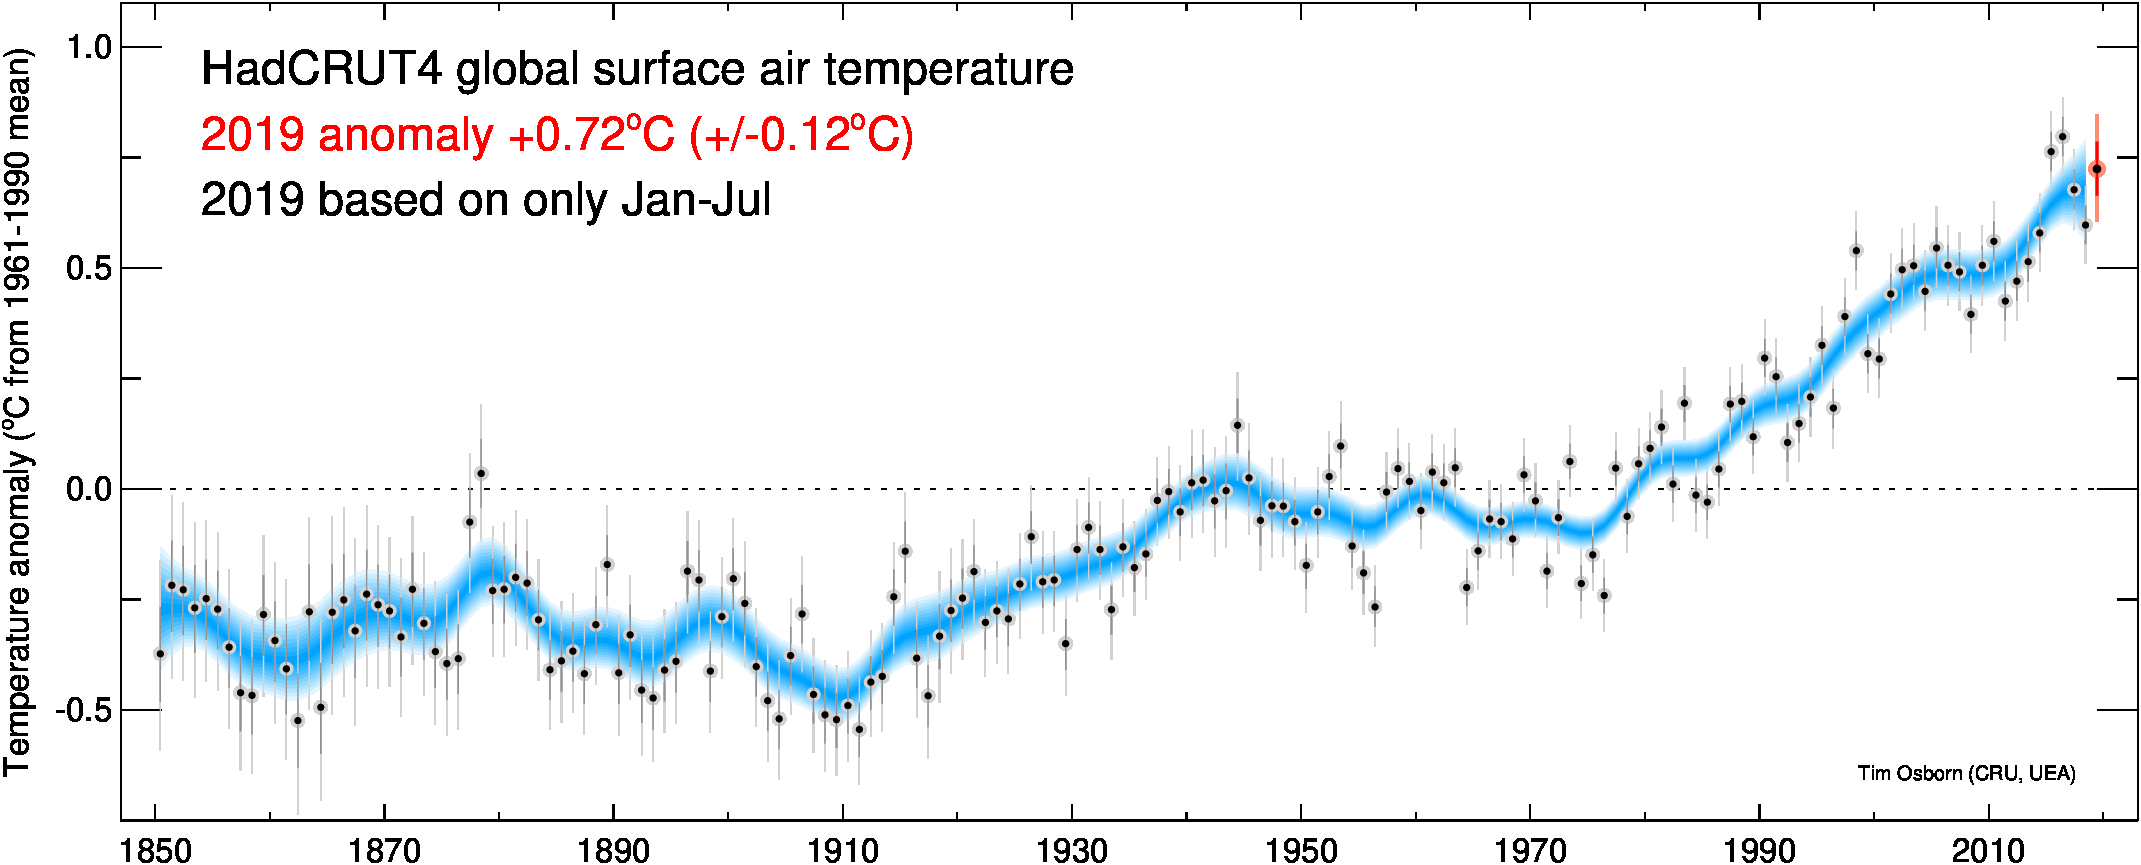
\includegraphics[scale=0.21]{average_temperature}}
\caption{Зависимость разности глобальной средней приповерхностной температуры воздуха и её среднего значения в период 1961-1990 гг. от времени}
\end{figure}

\item \textbf{Рост теплосодержания океана}
\newline
Океаны абсорбируют большое количество выделяющегося тепла. С 1969 г. температура верхних 700 м океана выросла более чем на $0,2 \degree C$ (Levitus et al, 2017).

\item \textbf{Рост уровня мирового океана} (вызванный термическим расширением воды при нагревании и таянием ледяного покрова)
\newline
Согласно данным Института космических исследований Годдарда (рис. 2), с 1993 года уровень мирового океана вырос на $(95 \pm 4) \; мм$. Текущая скорость увеличения уровня --- $(3,3 \pm 0,4) \; мм/год$. По данным австралийского Государственного объединения научных и прикладных исследований (рис. 3), с 1880 г. уровень океана вырос примерно на 230 мм.

\begin{figure}[h!]
\center{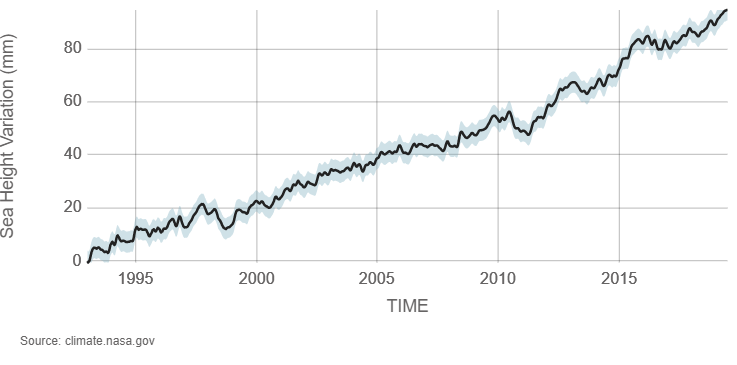
\includegraphics[scale=0.4]{SeaLevel}}
\caption{Зависимость изменения уровня мирового океана по сравнению с 1993 г. от времени}
\end{figure}

\begin{figure}[h!]
\center{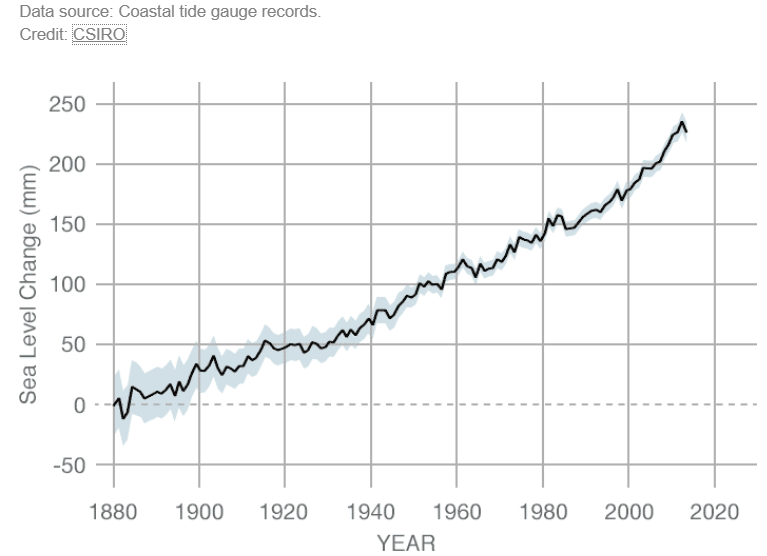
\includegraphics[scale=0.5]{SeaLevel1}}
\caption{Зависимость изменения уровня мирового океана по сравнению с 1880 г. от времени}
\end{figure}

\item \textbf{Уменьшение площади арктического морского льда}
\newline
Годовой минимум площади арктического морского льда достигается в сентябре. По данным NASA (рис. 4), в 1980 г. площадь сентябрьского льда составляла $7,67 \; млн \; км^{2}$, в 2019 г. --- $4,32 \; млн \; км^{2}$; 

\begin{figure}[h!]
\center{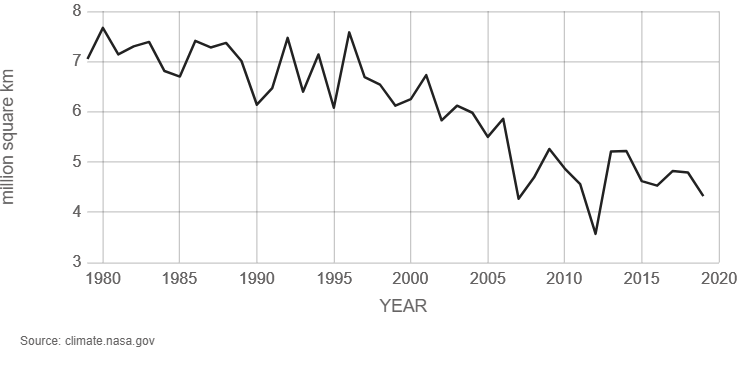
\includegraphics[scale=0.4]{SeaIce}}
\caption{Зависимость площади сентябрьского морского льда в Арктике от года}
\end{figure}

\item \textbf{Уменьшение ледяных покровов}
\newline
По данным NASA, Гренландия в среднем теряла 286 млрд тонн льда в год в период с 1993 по 2016 г., в то время как Антарктика в этот же самый период теряла в среднем 127 млрд тонн льда в год. При этом внутренние области Восточной Антарктики наращивают лёд, однако в целом она теряет его с ускоряющимся темпом.

\item \textbf{Увеличение концентрации углекислого газа в атмосфере}
Согласно данным Национального управления океанических и атмосферных исследований (рис. 5), в октябре 2019 г. концентрация углекислого газа в атмосфере составляла 412 ppm. Это самое большое значение величины как минимум за последние 400 тысяч лет (рис. 5).

\begin{figure}[h!]
\center{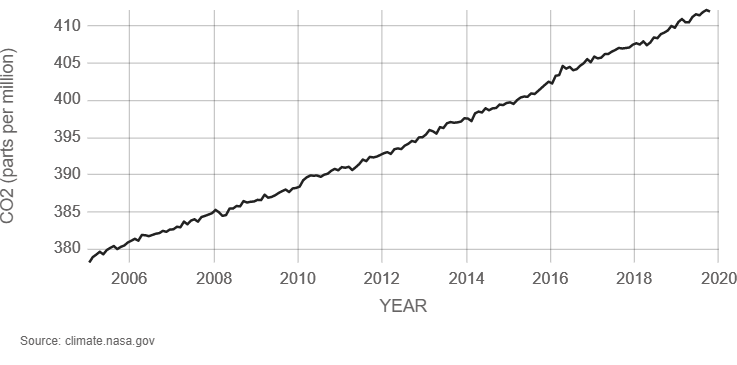
\includegraphics[scale=0.4]{CO2}}
\caption{Зависимость концентрации углекислого газа в атмосфере от времени с 2006 г.}
\end{figure}

\begin{figure}[h!]
\center{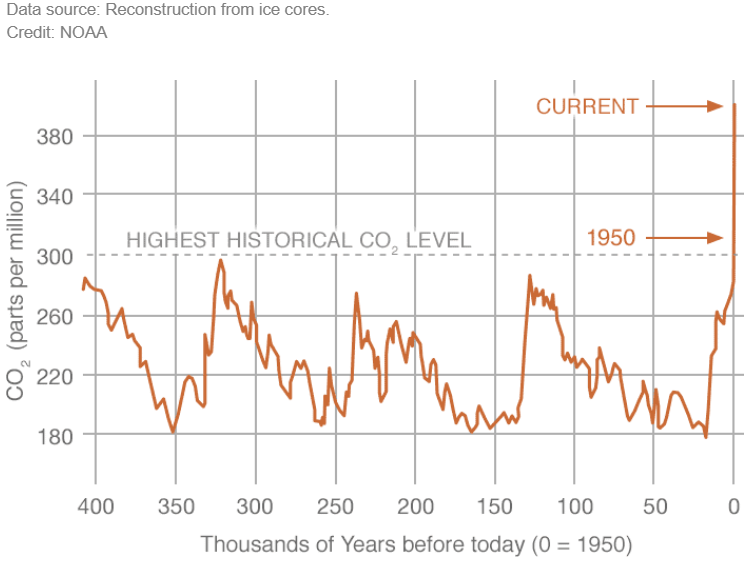
\includegraphics[scale=0.5]{CO2_long}}
\caption{Зависимость концентрации углекислого газа в атмосфере от времени за последние 400 тысяч лет}
\end{figure}

\end{enumerate}

В настоящее время подавляющее большинство специалистов-климатологов считают, что основная причина быстрого изменения климата --- деятельность человека (Cook et al, 2013). Вот некоторые факты, которые позволяют проследить эту связь:
\begin{itemize}
\item В атмосфере растёт количество углекислого газа --- сейчас оно почти в полтора раза превышает максимумы за последние 400 тысяч лет. 
\item Сжигание ископаемых топлив является основной причиной антропогенной эмиссии $CO_{2}$. В северном полушарии, где сжигается большая часть топлива, концентрация $CO_{2}$ выше, чем в южном.
\item Концентрация кислорода падает так, как было бы, если бы он полностью уходил на сжигание топлива.
\item В атмосферном углекислом газе становится относительно меньше изотопов углерода-14 и углерода-13, которых нет в нефти и угле.
\item $CO_{2}$ является парниковым газом.
\item Глобальная температура быстро растёт. При этом интенсивность солнечного излучения в последние 35 лет падает. Это и другие доказательства опровергают возможность связи нынешнего увеличения температуры с солнечной активностью, о которой говорят некоторые противники теории антропогенного изменения климата. Кроме того, некоторые учёные предполагают, что это уменьшение солнечной активности может быть началом "большого минимума" наподобие маундеровского. Однако в ряде статей (см. сноску 2, climate.nasa.gov/blog/2910/what-is-the-suns-role-in-climate-change/) делается вывод, что это может в лучшем случае на несколько лет замедлить вызванное человеком потепление.
\end{itemize}

Некоторые скептики говорят о том, что нынешнее потепление --- естественное явление, подобное случавшимся ранее в истории Земли. Сторонники теории антропогенной природы потепления отвечают следующим образом: естественные климатические изменения в прошлом подтверждают, что климат чувствителен к энергетическому дисбалансу. Если планета аккумулирует тепло, глобальные температуры будут расти. В настоящее время $CO_{2}$ вызывает энергетический дисбаланс благодаря парниковому эффекту. Изменения климата в прошлом на самом деле подтверждают чувствительность климата к $CO_{2}$, а увеличение количества $CO_{2}$ вызвано деятельностью человека.
\newline



\end{document}
